\documentclass[12pt,a4paper,english]{article}
\usepackage{times}
\usepackage[utf8]{inputenc}
\usepackage{babel,textcomp}
\usepackage{mathpazo}
\usepackage{mathtools}
\usepackage{amsmath,amssymb}
\usepackage{ dsfont }
\usepackage{listings}
\usepackage{graphicx}
\usepackage{float}
\usepackage{epsfig,floatflt}
\usepackage{subfig} 
\usepackage[colorlinks]{hyperref}
\usepackage[hyphenbreaks]{breakurl}
\usepackage[usenames,dvipsnames,svgnames,table]{xcolor}
\usepackage{textcomp}
\definecolor{listinggray}{gray}{0.9}
\definecolor{lbcolor}{rgb}{0.9,0.9,0.9}
\lstset{backgroundcolor=\color{lbcolor},tabsize=4,rulecolor=,language=python,basicstyle=\scriptsize,upquote=true,aboveskip={1.5\baselineskip},columns=fixed,numbers=none,showstringspaces=false,extendedchars=true,breaklines=true,
prebreak=\raisebox{0ex}[0ex][0ex]{\ensuremath{\hookleftarrow}},frame=single,showtabs=false,showspaces=false,showstringspaces=false,identifierstyle=\ttfamily,keywordstyle=\color[rgb]{0,0,1},commentstyle=\color[rgb]{0.133,0.545,0.133},stringstyle=\color[rgb]{0.627,0.126,0.941},literate={å}{{\r a}}1 {Å}{{\r A}}1 {ø}{{\o}}1}

% Use for references
%\usepackage[sort&compress,square,comma,numbers]{natbib}
%\DeclareRobustCommand{\citeext}[1]{\citeauthor{#1}~\cite{#1}}

% Fix spacing in tables and figures
%\usepackage[belowskip=-8pt,aboveskip=5pt]{caption}
%\setlength{\intextsep}{10pt plus 2pt minus 2pt}

% Change the page layout
%\usepackage[showframe]{geometry}
\usepackage{layout}
\setlength{\hoffset}{-0.6in}  % Length left
%\setlength{\voffset}{-1.1in}  % Length on top
\setlength{\textwidth}{480pt}  % Width /597pt
%\setlength{\textheight}{720pt}  % Height /845pt
%\setlength{\footskip}{25pt}

\newcommand{\VEV}[1]{\langle#1\rangle}
\title{FYS4150 - Project 2}
\date{}
\author{ Kristoffer Langstad\\ \textit{krilangs@uio.no}}

\begin{document}%layout
\maketitle
\begin{abstract}
In this project we want to solve eigenvalue problems of a tridiagonal Töplitz matrix using Jacobi's method. We will use unit tests to check our results with other solvers like Python's numpy. We will solve different physical problems by discretization and scaling to make them into similar differential equations that we solve numerically. The first problem is a classical wave function problem in one dimension as a two-point boundary value problem of a buckling beam. This eigenvalue problem has analytical solutions which we will use as a unit test against our numerical algorithm. We also check that the eigenvectors retain their orthogonality after the transformations. Both these tests passed and gave similar eigenvalues within a small tolerance of 1e-8. Next we look at a quantum mechanical problem for an electron in a 3-dimensional harmonic oscillator (quantum dots). This case also have analytical eigenvalues which we test against. For our numerical simulation we get eigenvalues $\lambda=[2.9998, 6.9990, 10.9976]$ for the first three eigenvalues, with 206'466 transformations for a $400\times400$ matrix and a $\rho_{max}=10$. For the last case we expand for two electrons which interact via a repulsive Coulomb interaction. Here we test for different frequency strengths $\omega_r=[0.01, 0.1, 1, 5]$ for the ground state. We find our numerical eigenvalues as $\lambda=[0.3116,2.2231, 4.0577,17.4436]$ for a $400\times400$ matrix and $\rho_{max}=10$, for their respective $\omega_r$. So here we see that another electron increases the energy levels and that it increases with increasing potential strength $\omega_r$.%For these frequencies there are analytical solutions that we compare our numerical ones with. 
\end{abstract}

\section{Introduction}
A hot topic in todays physics is what we call quantum dots where we look at electrons in small areas in semiconductors. To be able to solve this we have to look at differential equations. These are often difficult to solve analytically, and have to be solved numerically. Even then we have to do approximations to be able to make the equations easier to solve.

In our case we will use methods from linear algebra and look at eigenvalue problems. These are widely used to solve physical problems, so to understand how they work and how they are solved is important. Another powerful tool is to scale the equations. This means that we can solve an equation for one case, and then scale the equation to be able to solve it for another. This is one of the steps that we do in this project where we start with the wave equation for a buckling beam in one dimension, and then expand for a quantum mechanics case with the Schrödinger equation for the one and two electrons (quantum dots) in three dimensions case.

In the methods section we look at the theory we use and the implementation of the algorithms. We start with the buckling beam which is fastened in both ends, such that we know the endpoints with Dirichlet boundary conditions. The differential equations is simplified (scaled) with the introduction of a dimensionless variable $\rho$, such that we can discretize the new equation. This is now a eigenvalue problem that we will solve by solving a tridiagonal Töplitz matrix with Jacobi's method numerically. We then derive the algorithms to be used, and implement them and unit tests into a our program. Then we expand to quantum mechanics with the radial Schrödinger equation for one and two electrons in a three-dimensional harmonic oscillator potential. These equations are then manipulated and scaled to the form as the discretized buckling beam problem, but with other potential terms. For these cases we have analytical results to compare with. So the results of the eigenvalues are then compared to the analytical ones. We also look at the number of similarity transformations needed as a result of the matrix dimensionality and the maximum value of $\rho$. Lastly we come up with a conclusion to the project.

\section{Methods}
\subsection{Unitary transformation}
\label{sect_unitary_transf}
Consider a basis of vectors 
\[\textbf{v}_i = \begin{bmatrix}
v_{i1}\\
\vdots\\
v_{in}
\end{bmatrix}\]
which is orthogonal. This means that $\textbf{v}_j^T\textbf{v}_i=\delta_{ij}$. Then we define a unitary matrix $\textbf{U}$ such that $\textbf{U}\textbf{U}^T=\mathcal{I}$. A unitary transformation of the basis vector \textbf{v}$_i$ is then:
\begin{equation*}
\textbf{w}_i=\textbf{U}\textbf{v}_i
\end{equation*}
Then we take:
\begin{equation*}
\textbf{w}^T_j\textbf{w}_i=(\textbf{U}\textbf{v}_j)^T\textbf{U}\textbf{v}_i=\textbf{v}_j^T\textbf{v}_i\textbf{U}^T\textbf{U}=\textbf{v}_j^T\textbf{v}_i=\delta_{ij}
\end{equation*}
This is clearly orthogonal, which means that a unitary transformation preserves both the orthogonality and the dot product of the basis vector.

We can also check that the eigenvalues are preserved under a unitary transformation as seen in Computational Physics (7.3) \cite{lectures}:\\
Start with the eigenvalue problem and a similarity transformed matrix \textbf{B}. 
\begin{equation}
\label{eq:sim_transf}
\textbf{Ax}=\lambda\textbf{x}\quad \text{and}\quad \textbf{B}=\textbf{U}^T\textbf{A}\textbf{U}
\end{equation}
Multiply with \textbf{U}$^T$ and use that \textbf{U}$^T$\textbf{U}=$\mathcal{I}$:
\begin{align*}
\rightarrow (\textbf{U}^T\textbf{A}\textbf{U})(\textbf{U}^T\textbf{x})=\lambda\textbf{U}^T\textbf{x}\\
\Rightarrow \textbf{B}(\textbf{U}^T\textbf{x})=\lambda(\textbf{U}^T\textbf{x})
\end{align*}
Here we see that the eigenvalues are the same, but the eigenvectors have changed.

\subsection{Buckling Beam}
\label{sect:Beam}
First we have the classical wave equation in one dimension for the buckling beam problem with Dirichlet boundary conditions:
\begin{equation}
\label{eq:beam}
\gamma\frac{d^2u(x)}{dx^2}=-Fu(x), \quad x\in[0,L], \quad u(0)=u(L)=0
\end{equation}
$\gamma$ is a constant depending on properties of the beam with length $L$, $u(x)$ is the vertical displacement of the beam in $y$-direction and $F$ is the force acting on the beam. Then we introduce a dimensionless variable
\begin{equation*}
\rho=\frac{x}{L},\quad \rho\in[0,1],
\end{equation*}
into the differential equation \ref{eq:beam}. The new differential equation then looks like this:
\begin{equation}
\label{eq:beam_scale}
\frac{d^2u(\rho)}{d\rho^2}=-\frac{FL^2}{\gamma}u(\rho)=-\lambda u(\rho)
\end{equation}
This we discretize to an eigenvalue problem by using the second derivative of the function $u$ as
\begin{equation*}
\label{eq:u_2deriv}
u^{\prime\prime}=\frac{u(\rho+h)-2u(\rho)+u(\rho-h)}{h^2}+\mathcal{O}(h^2),
\end{equation*}
where $h$ is the step length defined, from the minimum value $\rho_{min}=\rho_0$ and maximum value $\rho_{max}=\rho_N$ for a given number of mesh points N, as
\begin{equation*}
h = \frac{\rho_N-\rho_0}{N}.
\end{equation*}
For a value of $\rho$ at a point $i$ we have $\rho_i=\rho_0+ih$ with $i=1,2,\cdots,N$. The differential equation \ref{eq:beam_scale} can now be rewritten with the second derivative $u^{\prime\prime}$, $\rho_i$ and $u(\rho_i)=u_i$ on compact form as
\begin{equation}
\label{eq:beam_discr}
-\frac{u_{i+1}-2u_i+u_{i-1}}{h^2}=\lambda u_i
\end{equation} 
As an eigenvalue problem we get
\begin{equation}
\label{eq:eigen_prob}
\begin{bmatrix}
d & a & 0 & \cdots & 0\\
a & d & a &\ddots & \vdots\\
0 & a & d & \ddots & 0\\
\vdots & \ddots & \ddots & \ddots & a\\
0 & \cdots & 0 & a & d
\end{bmatrix}
\begin{bmatrix}
u_1\\
u_2\\
\vdots\\
u_{N-2}\\
u_{N-1}
\end{bmatrix} = \lambda
\begin{bmatrix}
u_1\\
u_2\\
\vdots\\
u_{N-2}\\
u_{N-1}
\end{bmatrix},
\end{equation}
without considering the endpoints $u_0$ and $u_N$, and with $d=\frac{2}{h^2}$ and $a=-\frac{1}{h^2}$. This eigenvalue problem has analytical eigenpairs with eigenvalues as
\begin{equation}
\label{eq:analytic_eigenval}
\lambda_j = d+2a\cos(\frac{j\pi}{N+1}),\quad j=1,2,\cdots,N.
\end{equation}

\subsection{Jacobi's method}
\label{sect:Jacobi}
Now we implement the Töplitz matrix from the eigenvalue problem in equation \ref{eq:eigen_prob} into our program. This is dependent on the dimension of the matrix and the value for $\rho_{max}$ which we choose. Then we make a check of the matrix implementation where we compare the eigenvalues we get from the analytical eigenvalues in equation \ref{eq:analytic_eigenval} for a small Töplitz matrix (dimensions 5 or so) with Python's numpy.linalg.eig() for finding eigenpairs of the Töplitz matrix.

We are now going to solve the Töplitz matrix with Jacobi's method. The main idea with Jacobi's method is to do several similarity (unitary) transformations on the eigenvalue matrix in equation \ref{eq:eigen_prob}, till it is transformed to a diagonal matrix containing only the eigenvalues. The Jacobi rotation matrix 
\begin{equation}
\label{eq:jacobi_rotate}
\begin{bmatrix}
1 & 0 & \cdots & 0 & \cdots & 0\\
0 & \ddots & \vdots &\vdots & \vdots & \vdots\\
0 & \cdots & \cos\theta & \vdots & \sin\theta & \vdots\\
\vdots & \vdots & \cdots & 1 & 0 & \vdots\\
\vdots & \cdots & -\sin\theta & 0 & \cos\theta & 0 \\
0 & \cdots & 0 & \cdots & 0 & 1
\end{bmatrix}
\end{equation}
is an orthogonal ($n\times n$) transformation matrix that performs a plane rotation around the angle $\theta$ in Euclidean $n$-dimensional space \cite{lectures}(7.4). The angle $\theta$ is arbitrary and chosen such that all off-diagonal elements in \textbf{B} in equation \ref{eq:sim_transf} is zero. To do this we calculate the Frobenius norm of the matrix \textbf{A}, since the Frobenius norm is conserved under unitary transformations:
\begin{equation}
\label{eq:Frobenius}
||\textbf{A}||_F^2 = ||\textbf{B}||_F^2=\sum_{ij}|a_{ij}|^2=\sum_{ij}|b_{ij}|^2
\end{equation}
After taking the Frobenius norm we find the off-diagonal elements in \textbf{B} as:
\begin{equation}
\label{eq:off_diag}
off(\textbf{B})^2=||\textbf{B}||_F^2-\sum_{i=1}^{n}b_{ii}^2=off(\textbf{A})^2-2a_{kl}^2
\end{equation}
For each similarity transformation we can see that the matrix moves closer to diagonal form for each step. To do this numerically we implement a function for finding the maximum non-diagonal element value to start with, and this returns the position of the element to be used in the Jacobi rotation matrix. After one transformation the function finds the next maximum element. This continues until we are left with the diagonal matrix we want containing only the eigenvalues (or at least has non-diagonal elements smaller than a given tolerance $1e-8$). This function is implemented as:
\begin{lstlisting}
max_elem = 0
for i in range(n):
	for j in range(i+1, n):
		if abs(matrix[i,j]) > max_elem:
			max_elem = abs(matrix[i,j])
			max_k = i
			max_l = j
		else:
			pass
\end{lstlisting}
For simplification we define:
\begin{align*}
s = \sin\theta,\quad c=\cos\theta, \quad t=\tan\theta=\frac{s}{c}\quad \tau=\cot2\theta=\frac{a_{ll}-a_{kk}}{2a_{kl}}
\end{align*}
Here we define $\theta$ such that $a_{kl}\neq0$ for the non-diagonal elements of the transformed matrix. This yields the quadratic equation
\[t^2+2\tau t-1=0.\]
Where we easily find
\[t=-\tau\pm\sqrt{1+\tau^2},\quad c=\frac{1}{\sqrt{1+t^2}},\quad s=tc.\]
If we get a large value for $\tau$ we would get wrong results when calculating $t$. For large $\tau$ we could get a situation with $t\approx-\tau\pm\sqrt{\tau^2}$ which the computer would have to solve. This can give round-off errors. So we have to make a change that takes this case into consideration. We rewrite $t$ by its conjugate and implement it under a if-test:
\begin{lstlisting}
if tau >= 0:
	t = 1./(tau + np.sqrt(1. + tau**2))
else:
	t = -1./(-tau + np.sqrt(1. + tau**2))
\end{lstlisting}
For a similarity transformation like the one in equation \ref{eq:sim_transf}, where \textbf{U} is the rotation matrix in equation \ref{eq:jacobi_rotate} with the non-zero elements 
\begin{align*}
u_{kk} = u_{ll} &= c\\
u_{kl} = -u_{lk} &= -s\\
u_{ii} = -u{ii} &= 1\quad i\neq k\quad i\neq l,
\end{align*}
we can rewrite it as:
\begin{align*}
b_{kk} &= a_{kk} c^2 - 2a_{kl}cs + a_{ll} s^2\\
b_{ll} &= a_{kk} s^2 - 2a_{kl}cs + a_{ll} c^2\\
b_{kl} &= (a_{kk} - a_{ll})cs + a_{kl}(c^2-s^2)\\
b_{ik} &= a_{ik}c - a_{il}s, \quad i\neq k\quad i\neq l\\
b_{il} &= a_{ll}c + a_{ik}s, \quad i\neq k\quad i\neq l\\
b_{ii} &= a_{ii}, \quad i\neq k\quad i\neq l
\end{align*}
Here we have to choose the angle $\theta$ such that all $b_{kl}=0$ or smaller than a tolerance, which is what we do with the function for the maximum non-diagonal elements and the Jacobi rotation matrix. We also compute the eigenvectors for the matrix. For the solver for finding the eigenvalues we also take the time and number of transformations of the Jacobi rotation/maximum off-diagonal algorithm to compare for different matrix dimensions.

\subsection{Testing algorithms}
\label{sect:testing}
The main algorithms are found in the program \textit{main.py} in a GitHub-folder as found in Appendix \ref{sect:appendix} by following the link there. The programs for the testing of the algorithms we are about to explain are found in the same folder with name \textit{tests.py}. We test for small dimensions of matrices. For small matrices we can more easily control the expected results.

The first test we implement is a test of our matrix and the maximum non-diagonal element function. For this test we manually make a $5\times5$ matrix we random numbers. This is to easily check that the function can find the maximum non-diagonal element in the matrix. We also use a numpy function called \textbf{numpy.lib.stride\_tricks.as\_strided} to numerically find the maximum element in the matrix, and is only used to cross-check our function. Then we implement an error-call for if our function finds a diagonal element, or if finds another element which is not the same as for the numpy function.

Next we want to test that the eigenvalues we get from out constructed matrix in equation \ref{eq:eigen_prob} is correct. We calculate the analytical eigenvalues of the eigenvalue problem which is given in equation \ref{eq:analytic_eigenval}, and compare it with Python's \textbf{numpy.linalg.eig} of our constructed matrix. If they do not match within a tolerance of $1e-10$, we assert an error.

The last test we want to do is a test of Jacobi's method on our constructed Töplitz matrix. Here we want to check that we get the correct eigenpairs after the similarity transformations. First we check that Jacobi's method gives us the same eigenvalues as for the numpy function we used earlier, for any given square matrix of dimensionality we choose. If they do not match within a tolerance of $1e-8$, we assert an error. We can also take the time of the algorithm and see number of transformations if we choose so. Then we want to check that the orthogonality of the eigenvectors after transformations are preserved. To check this we take the inner product of the eigenvectors after the transformations. We set the test of orthogonality as successful if the inner products are smaller than a tolerance of $1e-8$. We check for the case if the element $i\neq j$ within the tolerance, and if the element $i=j$. If the tests fails, then we assert an error.

Another thing we do is to make some plots to see the dependency the matrix dimension has on the number of transformations needed and the time they take. All these plots can be seen in the Figures-folder in GitHub (\ref{sect:appendix}).

\subsection{Quantum dots, one electron}
\label{sect:quantum_one}
Next, we want to expand our numerics to a quantum mechanical problem for an electron moving in a three-dimensional harmonic oscillator potential. We will assume spherical symmetry, and will look at the radial part of Schrödinger's equation in spherical coordinate with $r\in[0,\infty)$:
\begin{equation}
\label{eq:rad_schr_1}
-\frac{\hbar^2}{2m}\left(\frac{1}{r^2}\frac{d}{dr}r^2\frac{d}{dr}-\frac{l(l+1)}{r^2}\right)R(r) + V(r)R(r)=ER(r)
\end{equation}
The potential for this case is the harmonic oscillator potential, $V(r)=\frac{1}{2}kr^2=\frac{1}{2}m\omega^2r^2$. The energy is then the corresponding harmonic oscillator energy with oscillator frequency $\omega$ as:
\begin{equation}
\label{eq:HO_energy_1}
E_{nl} = \hbar \omega\left(2n + l + \frac{3}{2}\right)
\end{equation}
$n=0,1,\cdots$ stands for which state we are looking at, while $l=0,1,\cdots$ is the orbital momentum of the electron. 

Then we do a substitution with $R(r)=\frac{1}{r}u(r)$ with boundary conditions\\ $u(0)=u(\infty)=0$ to get:
\begin{equation}
\label{eq:before_scale}
-\frac{\hbar^2}{2m}\frac{d}{dr^2}u(r)+\left(V(r)+\frac{l(l+1)}{r^2}\frac{\hbar^2}{2m}\right)u(r)=Eu(r)
\end{equation}

Now we want to scale the equation with a dimensionless variable $\rho=\frac{r}{\alpha}$, where $\alpha$ is a constant with dimension length. The harmonic oscillator potential is then $V(\rho)=\frac{1}{2}k\alpha^2\rho^2$. In this project we will use $l=0$. So now with the new potential and scaling, Schrödinger's equation is now:
\begin{equation*}
-\frac{\hbar^2}{2m\alpha^2}\frac{d^2}{d\rho^2}u(\rho)+V(\rho)u(\rho)=Eu(\rho)
\end{equation*}
Then we multiply the equation with $\frac{2m\alpha^2}{\hbar^2}$:
\begin{equation*}
-\frac{d^2}{d\rho^2}u(\rho)+\frac{mk}{\hbar^2}\alpha^4\rho^2u(\rho)=\frac{2m\alpha^2}{\hbar^2}Eu(\rho)
\end{equation*}
Since $\alpha$ is a constant, we can fix it however we want. So to make the equation easier we fix it to be:
\[\alpha=\left(\frac{\hbar^2}{mk}\right)^{\frac{1}{4}}\]
Then we can define one the right hand side, a variable for the eigenvalue of the problem as 
\[\lambda=\frac{2m\alpha^2}{\hbar^2}E.\]
The final Schrödinger equation that we have to solve has now become
\begin{equation}
\label{eq:fin_schr_1}
-\frac{d^2}{d\rho^2}u(\rho)+\rho^2u(\rho)=\lambda u(\rho).
\end{equation}

This now has the same type of form like the buckling beam problem in equation \ref{eq:beam_scale} just with another term. So we will do the exact same as we did earlier by discretization and a Taylor approximation to rewrite with the same $\rho_i=\rho_0+ih$. We have to use $\rho_{max}=\rho_N$ and not equal to $\infty$, since infinity cannot be represented numerically. So we can now rewrite the Schrödinger equation (\ref{eq:fin_schr_1}) as 
\begin{equation*}
-\frac{u(\rho_i+h)-2u(\rho_i)+u(\rho_i-h)}{h^2}+\rho_i^2u(\rho_i)=\lambda u(\rho_i).
\end{equation*}
In a more compact way we write:
\begin{equation}
\label{eq:schr_discr_1}
-\frac{u_{i+1}-2u_i+u_{i-1}}{h^2}+\rho_i^2u_i=-\frac{u_{i+1}-2u_i+u_{i-1}}{h^2}+V_iu_i=\lambda u_i
\end{equation}

In the buckling beam problem we had no potential working on it. In this problem we have the harmonic oscillator potential. This means that we have to add a potential term to the diagonal elements $d_i=\frac{2}{h^2}+V_i$, while the non-diagonal elements stays the same and are constants $e_i=-\frac{1}{h^2}$. Schrödinger's equation can then again be rewritten as
\begin{equation}
\label{eq:schr_eigen_1}
d_iu_i+e_iu_{i-1}+e_iu_{i+1}=\lambda u_i.
\end{equation}
This equation can be written as a symmetric matrix eigenvalue problem just like equation \ref{eq:eigen_prob}, where we have left out the endpoints 0 and $N$.

As we can see, our eigenvalue problem for the electron has the same form and is solved in the same way as for the buckling beam problem numerically. The only thing we do is to add the harmonic oscillator potential to the diagonal elements. So now we can experiment with the dimensionality of the matrix and the value of $\rho_{max}$. We want to find optimal values for the dimensionality and $\rho_{max}$ such that the eigenvalues we get are close enough to the analytical eigenvalues $\lambda=3,7,11,15,...$ with 3-4 leading digits after the decimal. We also look at the number of integration points needed to produce these results. The eigenvalues for the three lowest-lying states are then plotted for the optimal values.

\subsection{Quantum dots, two electrons}
\label{sect:quantum_two}
Once again we will expand our problem. Now we add another electron to the harmonic oscillator well. These two electrons interact with each other by a repulsive Coulomb interaction. We start with the following radial Schrödinger's equation for one electron:
\begin{equation}
\label{eq:schr_single_2}
-\frac{\hbar^2}{2m}\frac{d^2}{dr^2}u(r)+\frac{1}{2}kr^2u(r)=E^{(1)}u(r)
\end{equation}
Then for two electrons with no interaction and the two-electron energy $E^{(2)}$, we get
\begin{equation}
\label{eq:schr_double_2}
\left(-\frac{\hbar^2}{2m}\frac{d^2}{dr_1^2}-\frac{\hbar^2}{2m}\frac{d^2}{dr_2^2}+\frac{1}{2}k(r_1^2+r_2^2)\right)u(r_1,r_2)=E^{(2)}u(r_1,r_2).
\end{equation}
Now $u(r_1,r_2)$ is a two-electron wave function. Since we do not have an interaction between the electrons here, this can be taken as the product between two single-electron wave functions.

To simplify the equation we introduce the center-of-mass coordinate $\textbf{R}=\frac{1}{2}(\textbf{r}_1+\textbf{r}_2)$ and the relative coordinate $\textbf{r}=\textbf{r}_1-\textbf{r}_2$. This makes it possible to solve the equation as a single body problem, instead of a two-body problem which is more difficult. Schrödinger's equation with these coordinates becomes
\begin{equation}
\label{eq:schr_CM}
\left(-\frac{\hbar^2}{m}\frac{d^2}{dr^2}-\frac{\hbar^2}{4m}\frac{d^2}{dR^2}+\frac{1}{4}kr^2+kR^2\right)u(r,R)=E^{(2)}u(r,R).
\end{equation}

Next we separate the wave function as $u(r,R)=\psi(r)\phi(R)$ and with the two-electron energy as $E^{(2)}=E_r+E_R$, where $E_r$ is the radial energy and $E_R$ is the center-of-mass energy. Then by adding the Coulomb interaction as 
\[V(r_1,r_2)=\frac{\beta e^2}{r},\quad \beta e^2=1.44 \text{ eVnm},\]
to Schrödinger's equation (\ref{eq:schr_CM}) we obtain the $r$-dependent term as
\begin{equation}
\label{eq:shcr_split_2}
\left(-\frac{\hbar^2}{m}\frac{d^2}{dr^2}+\frac{1}{4}kr^2+\frac{\beta e^2}{r}\right)\psi(r)=E_r\psi(r).
\end{equation}

This is similar to equation \ref{eq:before_scale}, so we introduce again the dimensionless variable $\rho$ and do the same calculations as before. We end up with 
\begin{equation}
\label{eq:before_alpha_2}
-\frac{d^2}{d\rho^2}\psi(\rho)+\frac{mk}{4\hbar^2}\alpha^4\rho^2\psi(\rho)+\frac{m\alpha\beta e^2}{\rho\hbar^2}\psi(\rho)=\frac{m\alpha^2}{\hbar^2}E_r\psi(\rho).
\end{equation}
Now we define a new frequency term
\[\omega_r^2=\frac{mk}{4\hbar^2}\alpha^4,\]
and fix $\alpha$ to be
\[\alpha=\frac{\hbar^2}{m\beta e^2}.\]
Then we define the eigenvalues for the problem as 
\begin{equation}
\label{eq:eigenval_2}
\lambda=\frac{m\alpha^2}{\hbar^2}E.
\end{equation}
The final Schrödinger equation to be solved is now
\begin{equation}
\label{eq:final_schr_2}
-\frac{d^2}{d\rho^2}\psi(\rho)+\omega_r^2\rho^2\psi(\rho)+\frac{1}{\rho}=\lambda\psi(\rho).
\end{equation}

We want to study the problem for several values of the oscillator frequency\\ $\omega_r=[0.01, 0.5, 1, 5]$ for the ground state ($l=0$), which we now consider as the strength of the oscillator potential. In this case we also have to find the optimal/stable values for the dimensionality and $\rho_{max}$ for the $\omega_r$ values. Since the Schrödinger equation we have obtained is on the form as the two previous cases, we reuse our code but now with a new potential $V(\rho)=\omega_r^2\rho^2+\frac{1}{\rho}$. Then we look at our eigenvalues (and compare with the analytical calculations from M.Taut \cite{analytiv_eigval}) for the ground states, and plot the ground state for the different $\omega_r$'s.

\section{Results}
For our testing of the buckling beam we chose to run for smaller matrices. This is because smaller matrices need fewer similarity transformations and does not take a lot of time. With our code, all the tests in \textbf{tests.py} were successful. Thus, nothing was printed when we ran the program, other than printouts to verify that all the tests actually started. The output can be seen at the bottom of the code.

Then we wanted to see how the run-time and number of transformations needed to reduce the Töplitz matrix to a diagonal eigenvalue matrix, were affected by the dimension of the matrix. In the folder "Figures", which you find by going to the GitHub-link in Appendix \ref{sect:appendix}, lies plots for the time taken for the similarity transformations and the number of transformations as functions of the matrix dimensionality. We have plotted three different types for each of the two cases; 
\begin{itemize}
	\item log-log plot, where we get a linear growth in both cases.
	\item semi-log plot, where we see there are a high increase in time and transformations for the first couple of hundred dimensions before it starts to flatten more out as the dimensionality increases.
	\item a "normal" plot as seen in Figure \ref{fig:time_transf}, where we see that the curve has a almost an exponential growth with few transformations and short times for the first couple of hundred dimensions
\end{itemize}
\begin{figure}[htbp]
	%\hspace*{-2.5cm}
	\subfloat[Plot of the time of the transformations as function of dimensionality]{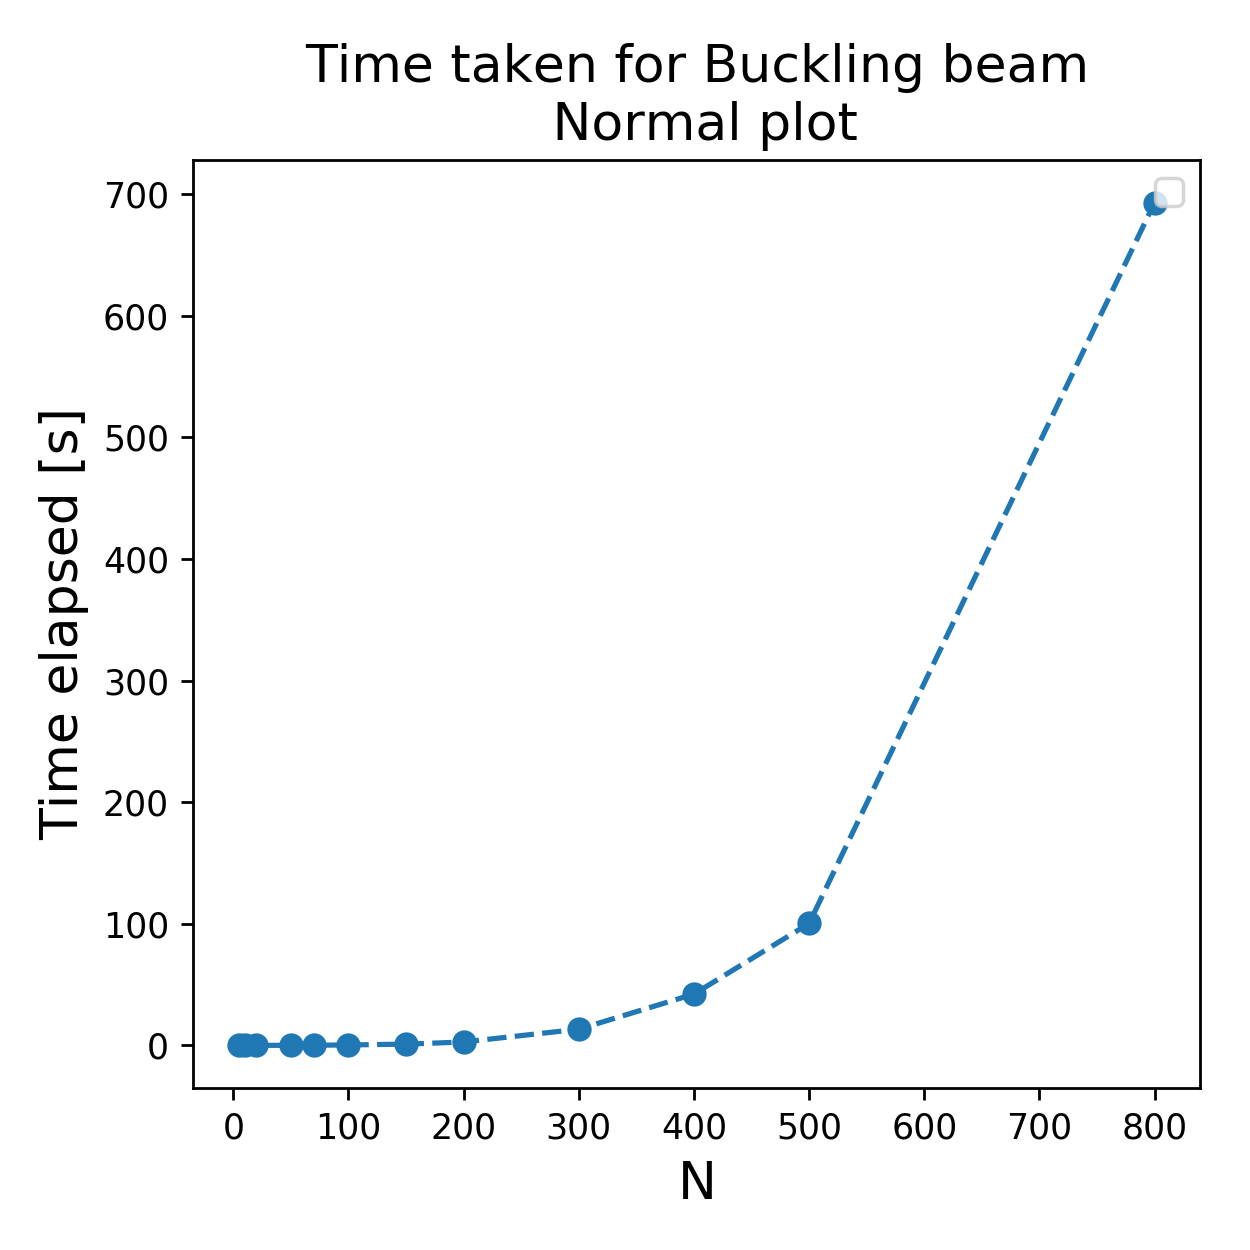
\includegraphics[width=0.5\linewidth]{Time_plot.png}}
	\subfloat[Plot of the number of transformations as function of dimensionality]{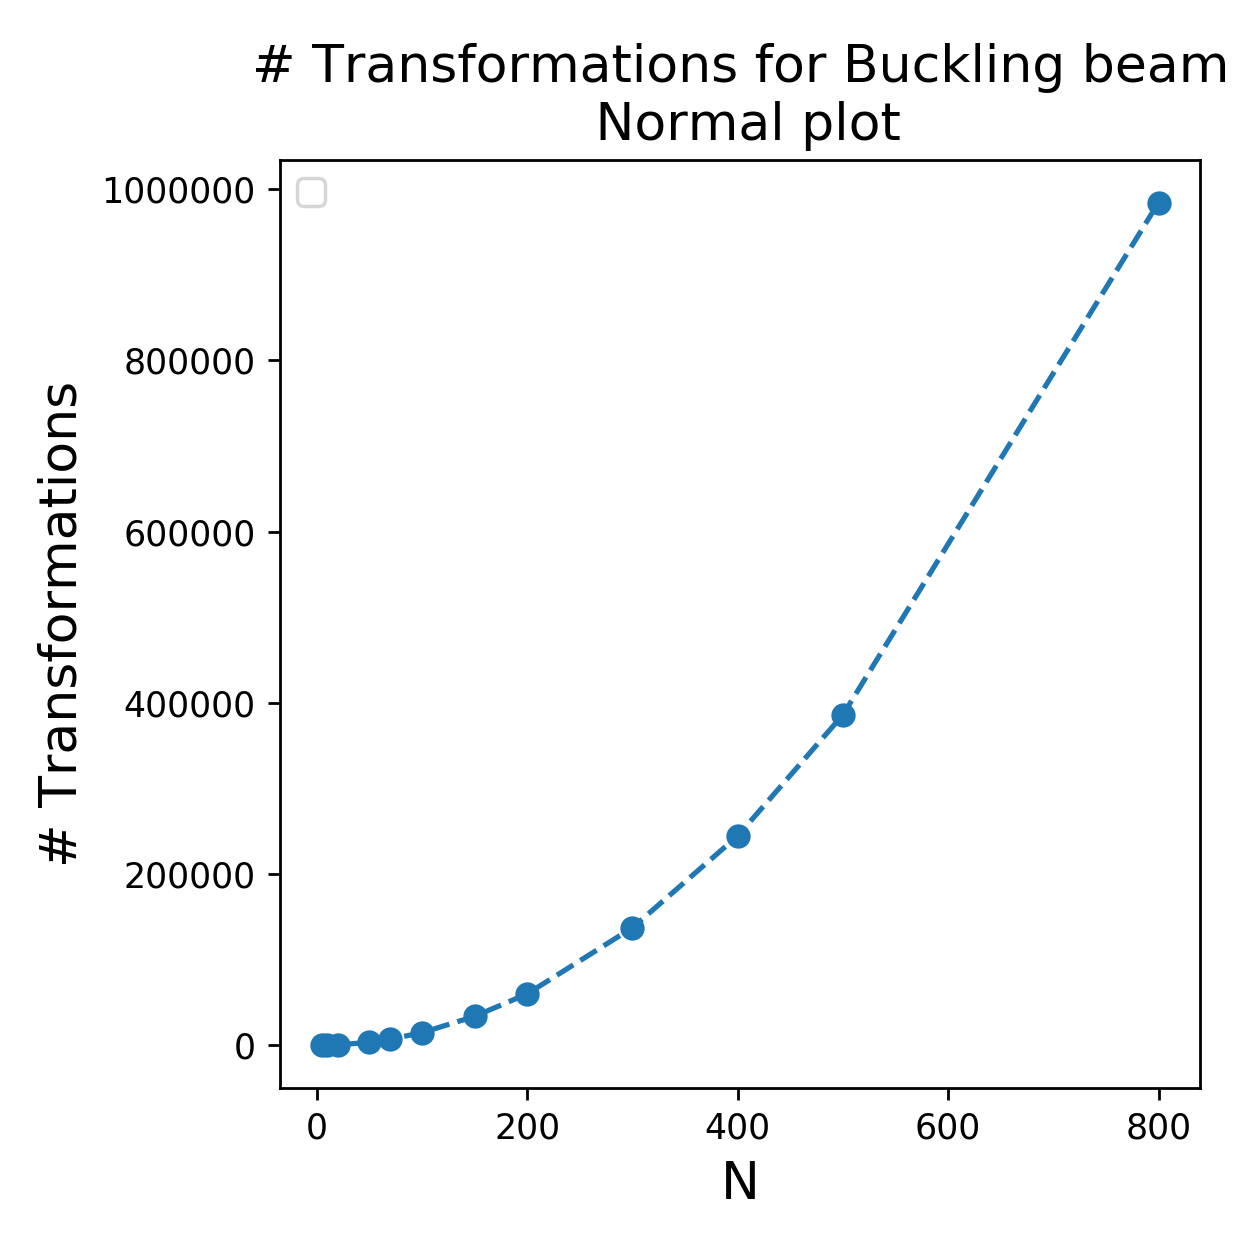
\includegraphics[width=0.5\linewidth]{Transformations_plot.png}}
	\caption{To the left we see a plot of the time of the Jacobi method for reducing the Töplitz matrix to an eigenvalue diagonal matrix as a function of the matrix dimensionality. To the right we see a plot of the number of transformations as a function of matrix dimensionality needed to reduce the Töplitz matrix by use of the Jacobi method. EXPLANATION::\label{fig:time_transf}}
\end{figure}

\section{Conclusion}

\appendix
\section{Appendix}
\label{sect:appendix}
Link to GitHub repository:

\begin{thebibliography}{}
\bibitem[1]{lectures}
Hjorth-Jensen, M. (2015). \textit{Computational Physics, Eigensystems chap. 7}

\bibitem[2]{analytiv_eigval}
Taut, M. Phys. Rev. A 48, 3561 (1993), \textit{Two electrons in an external oscillator potential: Particular analytic solutions of a Coulomb correlation problem}\\
\url{https://journals.aps.org/pdf/abstract/10.1103/PhysRevA.48.3561}
\end{thebibliography}
\end{document}

%This equation for no interaction between two electrons has analytical eigenvalues \cite{analytiv_eigval} calculated as
%\begin{equation*}
%\lambda_m = V_0 + \omega_e\left(m+\frac{1}{2}\right),
%\end{equation*}
%where $m=0,1,2,...$ and
%\begin{align*}
%V_0&=\frac{3}{2}\left(\frac{\omega_r}{2}\right)^{\frac{2}{3}}\\
%\omega_e&=\sqrt{3}\omega_r.
%\end{align*}
%So the eigenvalues are:
%\begin{equation}
%\label{eq:analytic_eigval_2}
%\lambda_m=\omega_r\left(2m+\frac{3}{2}\right)
%\end{equation}
%In the analytical calculations from M.Taut \cite{analytiv_eigval}, there is kept a factor $0.5$ that we have to multiply out for our numerical results to match.
